\documentclass{article}
\usepackage{amsmath,textcomp,amssymb,geometry,graphicx,enumerate}

\def\Name{Ran Liao}  % Your name
\def\SID{3034504227}  % Your student ID number
\def\Homework{2} % Number of Homework
\def\Session{Spring 2019}

\title{Explanation for Project 1}
\author{\Name, SID \SID}
\markboth{CS161--\Session\ }{CS161--\Session\ }
\pagestyle{myheadings}
\date{\today}

\textheight=9in
\textwidth=6.5in
\topmargin=-.75in
\oddsidemargin=0.25in
\evensidemargin=0.25in

\begin{document}
\maketitle

\section{Behind the Scenes}

Function $deja\_vu()$ uses $gets()$ to receive input from user without checking array bound properly. Therefore, a long input string can easily overwrite the return address in $deja\_vu()$ stack frame. 

\begin{figure}[h]
\centering
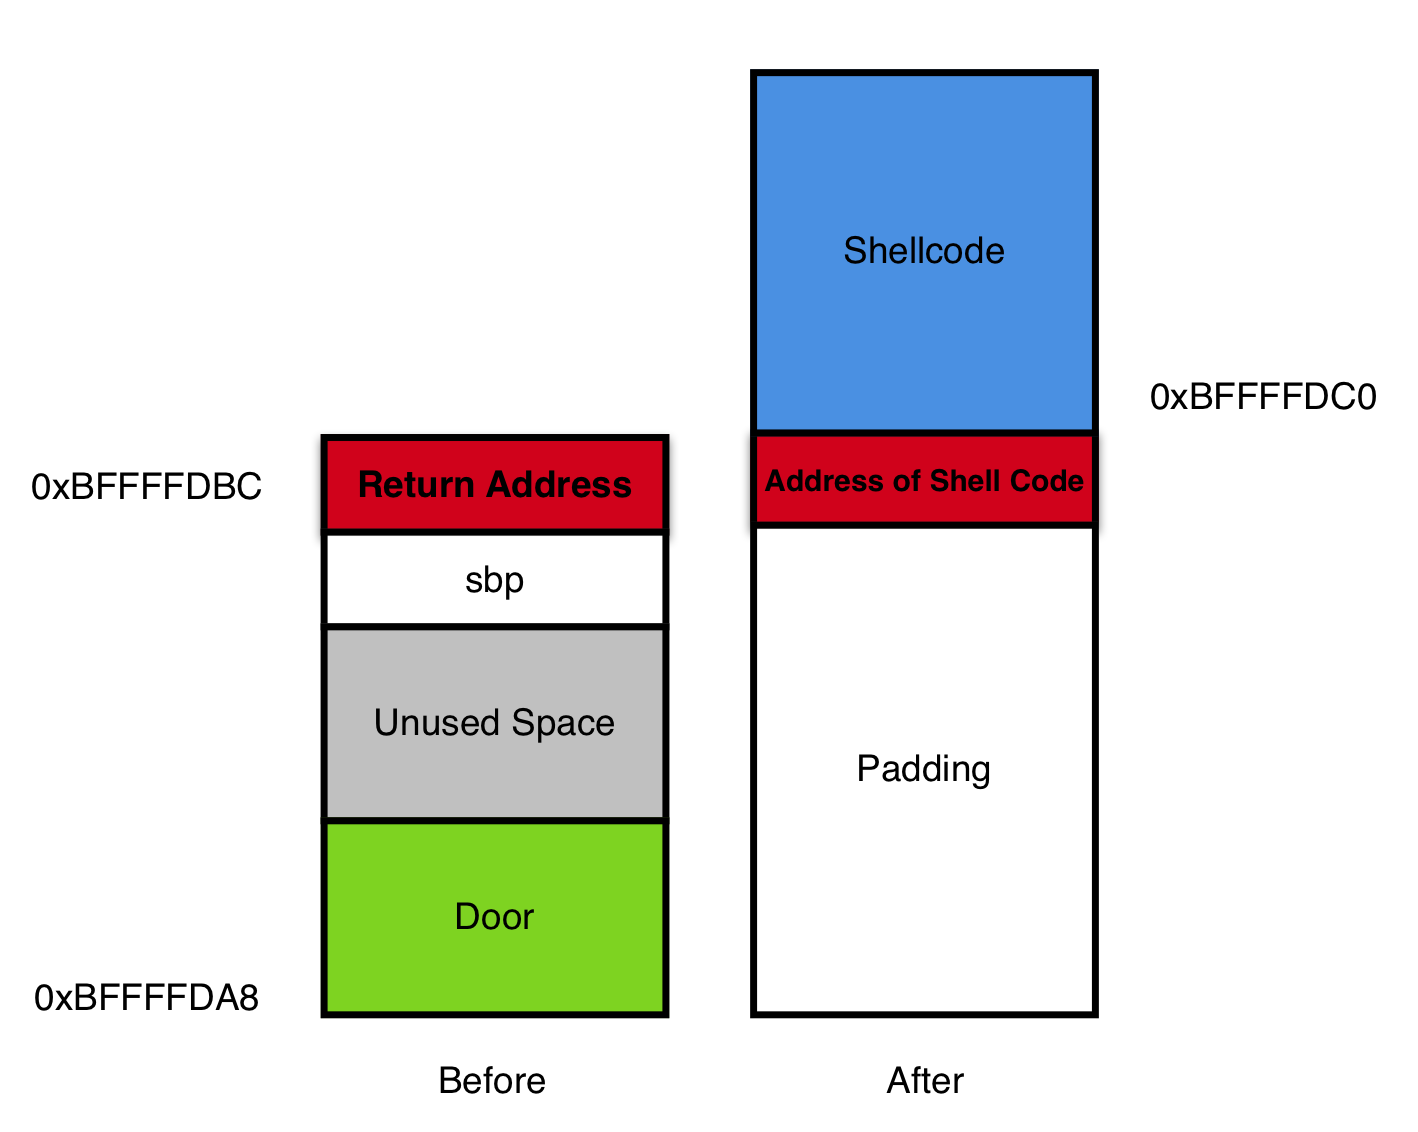
\includegraphics[width=0.5\textwidth]{stack1.png}
\caption{\label{fig:stack1}Stack Layout}
\end{figure}

Figure \ref{fig:stack1} demonstrates the memory layout of this buggy program. $Door$ is a 16-bytes buffer, $sbp$ is a 4 bytes integer, and there're another 16 bytes padding between them. In total, malicious input should start with 20 bytes padding. Then, the value of 0xBFFFFDC0 will be written to the next location. This is where the return address be stored. And this value is actually the address right behind this location, in which the malicious shellcode will be injected. 

The address of $sbp$ can be retrieved by letting gdb print the value of $ebp$ register. Add 4 to it will get the correct address that need be written during overflow process.

\begin{figure}[h]
\centering
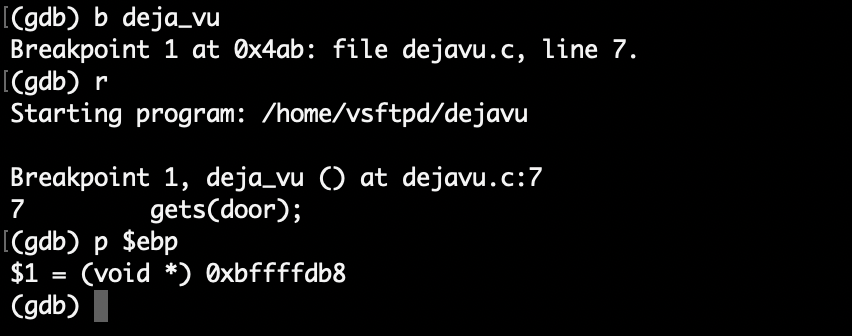
\includegraphics[width=0.5\textwidth]{gdb1.png}
\caption{\label{fig:gdb1}Retrieve Memory Address}
\end{figure}

\newpage
\section{Compromising Further}

This program uses \textbf{char} to receive an integer that used to check array access boundary. However, \textbf{char}
 is a signed data type, which means it can be negative. Thus by passing a negative value to it, e.g., 0xFF, we can bypass the boundary checking and initiate an overflow attack.
 
 \begin{figure}[h]
\centering
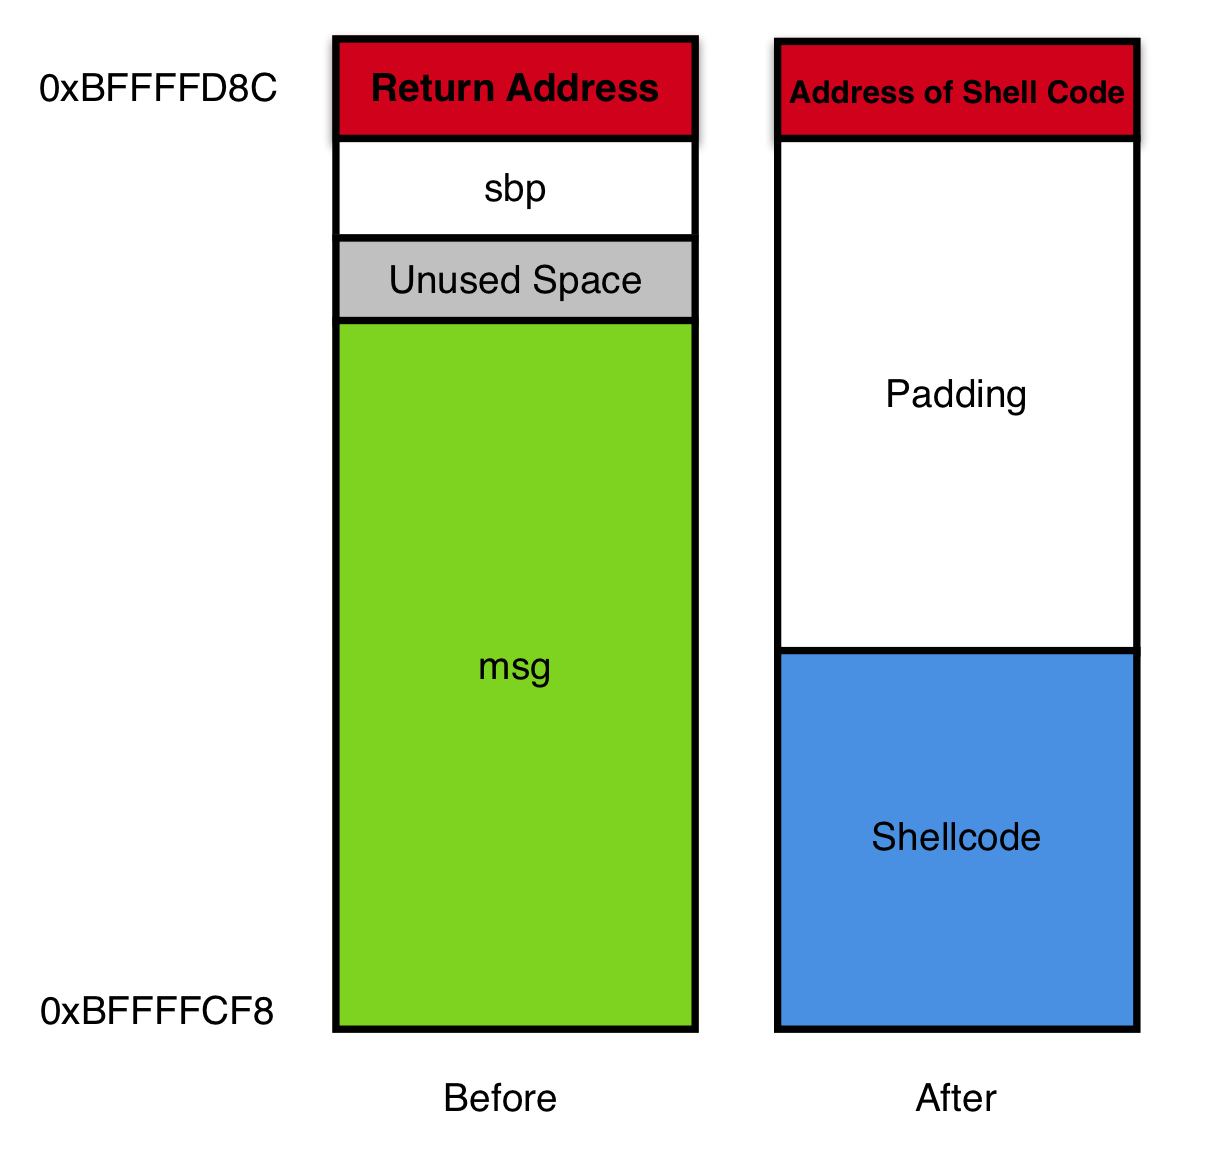
\includegraphics[width=0.5\textwidth]{stack2.png}
\caption{\label{fig:stack2}Stack Layout}
\end{figure}

The first byte of my malicious input is 0xFF, which is used to bypass the boundary checking. $msg$ is a 128-bytes long buffer, which have enough space to put the shellcode. Then, another 105 bytes no-sense padding is introduced. As figure \ref{fig:stack2} demonstrates, the next location is the return address we need to overwrite. The correct value is 0xBFFFFCF8. This is the address of variable $msg$ as well as where the shellcode is put. It's position relative to $sbp$ can be calculated by reading assembly codes carefully, and the address of $sbp$ can be printed by gdb.

\begin{figure}[h]
\centering
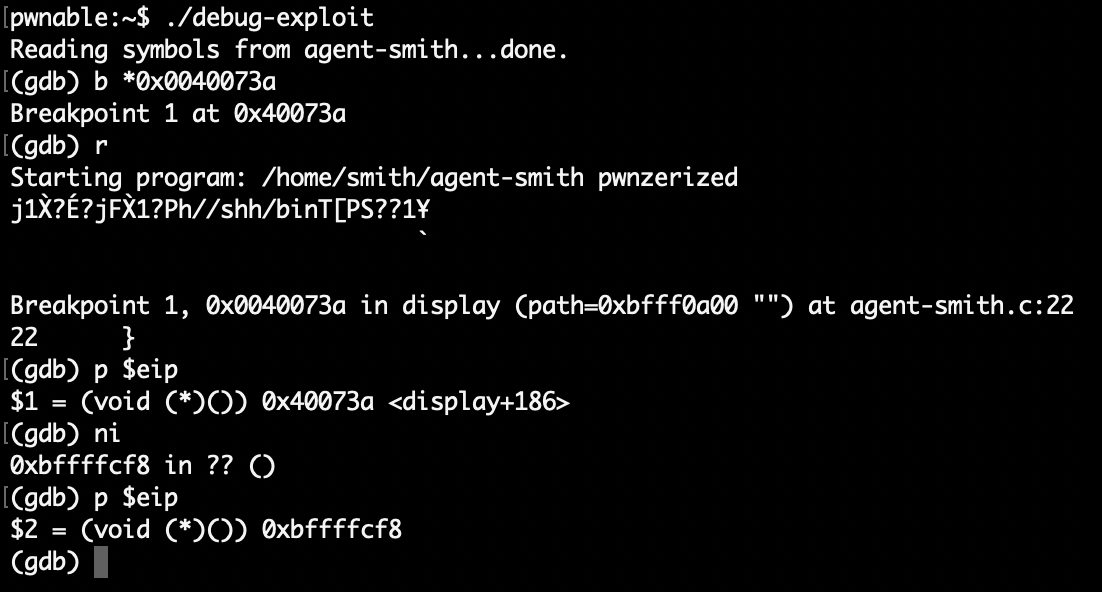
\includegraphics[width=0.7\textwidth]{gdb2.png}
\caption{\label{fig:gdb2}EIP value}
\end{figure}

In figure \ref{fig:gdb2}, I use gdb to print the value in $eip$ register. As you can see, it changed to 0xBFFFFCF8, which means I hijacked the control flow.

\newpage
\section{Deep Infiltration}


\end{document}